\subsection{General Strategy Overview}
This could also be an introductionary text which motivates the following subsections.

%%%%%%%%%%%%%%%%%%
\subsection{Agent Specific Strategies}
How are the agents specialised? Explorers keep probing for long. Inspectors probe enemies so that we can avoid saboteurs. Saboteurs are attacking and can be called for zone defence. Disabled agents communicate with repairers and approach them. Depending on how short this or the ``General Strategy Overview'' section is going to be, they could be merged.

%%%%%%%%%%%%%%%%%%
\subsection{DSDV}
What is it? How is it used in our context? What are advantages we gain from it? What is problematic (speed loss)?

%%%%%%%%%%%%%%%%%%
\subsection{Exploration}
How do agents move around during the exploration phase?

%%%%%%%%%%%%%%%%%%
\subsection{Zone Forming}
% TODO: update this according to how the subsection will be in the end
Zoning is the most important part in the MAPC Mars scenario~\cite{ahlbrecht_mapc_2014}.% p.3
It describes the process of agents occupying nodes in a way that they enclose a subgraph. In subsection~\ref{alg:zon_roles} we introduce two additional agent roles which are assigned during zoning. Said roles define the tasks and duties of an agent in this phase.

For our approach, zoning should take place after the map exploration phase. This should ensure that enough information about the map has been gathered to calculate high valuable zones close to the agents' current positions. The algorithm for finding these zones and determining which agents have to occupy which nodes is presented in subsection~\ref{alg:zon_colouring}.

The process of forming a zone and the associated agent communication is presented in the last subsection~\ref{alg:zon_formation}. It features the assignment of zone roles to agents. Furthermore, it is illustrated what zone is to be built and what the agents have to do to achieve this.

\subsubsection{Zone Construction}\label{alg:zon_construction}
The graph coloring algorithm used by the MAPC server to determine occupied zones is described in detail in the scenario description (\texttt{scenario.pdf}) included in the 2014 MAPC download package and will not be explained again here. To position themselves in an optimally-scoring way, agents could use the same algorithm on their side to calculate the agent placement that will lead to the highest total sum of zone scores in each step. However, the number of ways to place $n$ agents on $k$ nodes is $C \left (n+r-1,r-1\right )= \frac{\left(n+r-1 \right )!}{n!\left(r-1 \right )!}$, a number that increases rapidly with $n$ and $k$. In particular, there are $C \left (28+600-1,600-1 \right ) = 3.7463887025070038e+48$ ways to place 28 agents on 600 nodes - far too many to calculate in real-time.

\iffalse % comments out the following
Due to the way the server-side colouring algorithm works, placing $N$ agents on the map so that they establish the highest possible zone value per step is anything but straight-forward. Even for $n = 1$, a single agent placed on an articulation point in the graph can establish a high-value zone if there are no enemy agents in either subgraph that it splits the map into. \autoref{fig:articulation_points} shows an example.
\begin{figure}
  \centering
  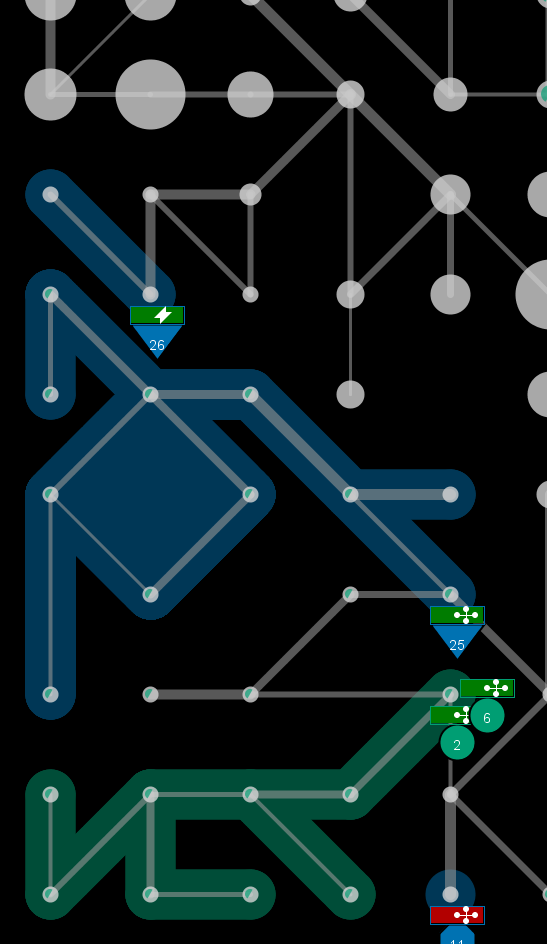
\includegraphics[width=\gri\textwidth]{articulation_points}
  \caption{The control loop for the agent deliberation process in the BOID architecture. Taken from \citeauthor{broersen2002goal}~\cite{broersen2002goal}.}
  \label{fig:control}
\end{figure}
In some way, we try to find local maxima to build small zones with as few agents as possible. How do we find zones? How do we find out how many agents we need? Explain that extending zones describes how the score resulting from an active zone can be increased by using idle agents. How do we determine what additional spots for zone extensions exist?
Present our colouring algorithm and the concept of a centre node.
\fi

\subsubsection{Zone Negotiation}\label{alg:zon_formation}
Zoning happens asynchronously. Who registers when for zoning? How do they unregister?
How do agents decide what zone to form? Which agents become coaches and which become minions? How do agents know which node they have to occupy?

\subsubsection{Zoning Roles}\label{alg:zon_roles}
This subsection describes the two roles exclusive to zoning and their associated tasks and duties throughout the lifecycle of a zone. These roles are those of a \emph{coach} and a \emph{minion}. Each zone is built by one coach and a varying amount of minions. Minions are agents which are dedicated to build a zone by obeying their coach's orders. Every agent may only be part of one zone at a time. % The last sentence is probably redundant.
The roles are assigned when a concrete zone is about to be built. Zoning agents keep either of these roles until the zone is broken up or they have to leave it. The roles regulate the agents' behaviour throughout the time they spend in a zone.

% This subsection describes the communication hierarchy during active zoning until its breakup

% TODO unregister from zoning
Before looking at border cases, an ideal case of a zone lifecycle is presented. There, the zone negotiation described in subsection~\ref{alg:zon_formation} ends with all agents knowing about the same best zone. This zone was found by one agent which will then become the zone's coach. Next, the coach informs the agents which will be part of the zone where to go to. On receipt of this message, the agents become minions and move to their designated node. The coach will also have to move to his node, which happens to be the centre node of the zone.
In a zone, minions serve no other purpose than to occupy their designated node. If a minion becomes disabled, he has to move towards a repairer. Due to this, he has to leave his node. Therefore, the zone can no longer exist in its original form. In such a case, a minion has to inform his coach about his departure. The coach must then tell all his other minions that the zone can no longer be maintained. Consequential, all affected agents drop their role and restart looking for zones as illustrated in subsection~\ref{alg:zon_formation}.

In reality, the zoning process is asynchronous. Therefore, it is likely that some agents start looking for a zone when others have nearly finished. Since a result, there can be multiple groups of agents with different knowledge about which zone would currently bring the highest score per agent. Each group could then be expecting a different agent to become a coach. This interferes with the assumptions that each agent may only be in one zone and have only one role at a time. As a solution, coaches do not only inform their minions about where to move to. Instead, they also transmit the per agent score of the zone they want to build together with this agent. Any agent can then compare the received zone score with the zone it wanted to build before. If it is higher, he must inform the coach of his former zone or his minions if he had been the coach himself. In case that the proposed zone's score is lower than the zone the agent intended to form, he must inform the coach who just proposed the new zone. Said coach will then have to inform all his minions that his zone is not going to be built.

Besides coaches and minions, there are also other agents who might be looking for a zone but will not be part of the one which will be built. Such an agent should not simply wait until a new zone is built. Instead, he should look for any highly valuable node in his surrounding which is not yet occupied by anyone. The range to look for such a node is the same as with the range for finding a zone in the agents neighbourhood presented in section~\ref{alg:zon_colouring}. It is increased after every zone finding process which does not result in a zone where the agent is part of. The idea is that with a wider range, the probability to find a highly valuable zone increases. Additionally, the agent will likelier move farther away from his position in case he is not part of the zone to be built. This should further ensure that the same zones are only proposed multiple times as best zones if they have a very high per agent score.

We assume due to our colour algorithm for zone finding that a node within a zone will be occupied by at most one agent. Then, any enemy agent close by a zone endangers it. This is because a zone may not spread across an enemy inside of it~\cite{ahlbrecht_mapc_2014}. % p.12
Furthermore, enemy saboteurs can disable zoning agents, which similarly destroys the zone in its original form~\cite{ahlbrecht_mapc_2014}. % p.11
Hence, coaches check once per step whether an enemy agent is close to the zone. If this is the case, the coach broadcast a message to all saboteurs to come and defend the zone. The saboteurs bid for this with the closest saboteur to the zone's centre winning. He will then move towards the enemy to disable him. If the coach detects in a next step that the enemy moves away from the zone, he will cancel the zone defence through another broadcast.


% below here are notes for things to mention:
% There are coaches and minions. Coaches command minions. There are also agents who don't get assigned a specific role and try to find and go to a well. There is a strict hierarchy between the roles.
